% C8. Pesos por parecido con test
\begin{frame}{Le enseñamos al modelo a mirar lo que se parece a Chapinero}
  \begin{columns}[c]
    \begin{column}{0.5\textwidth}\centering
      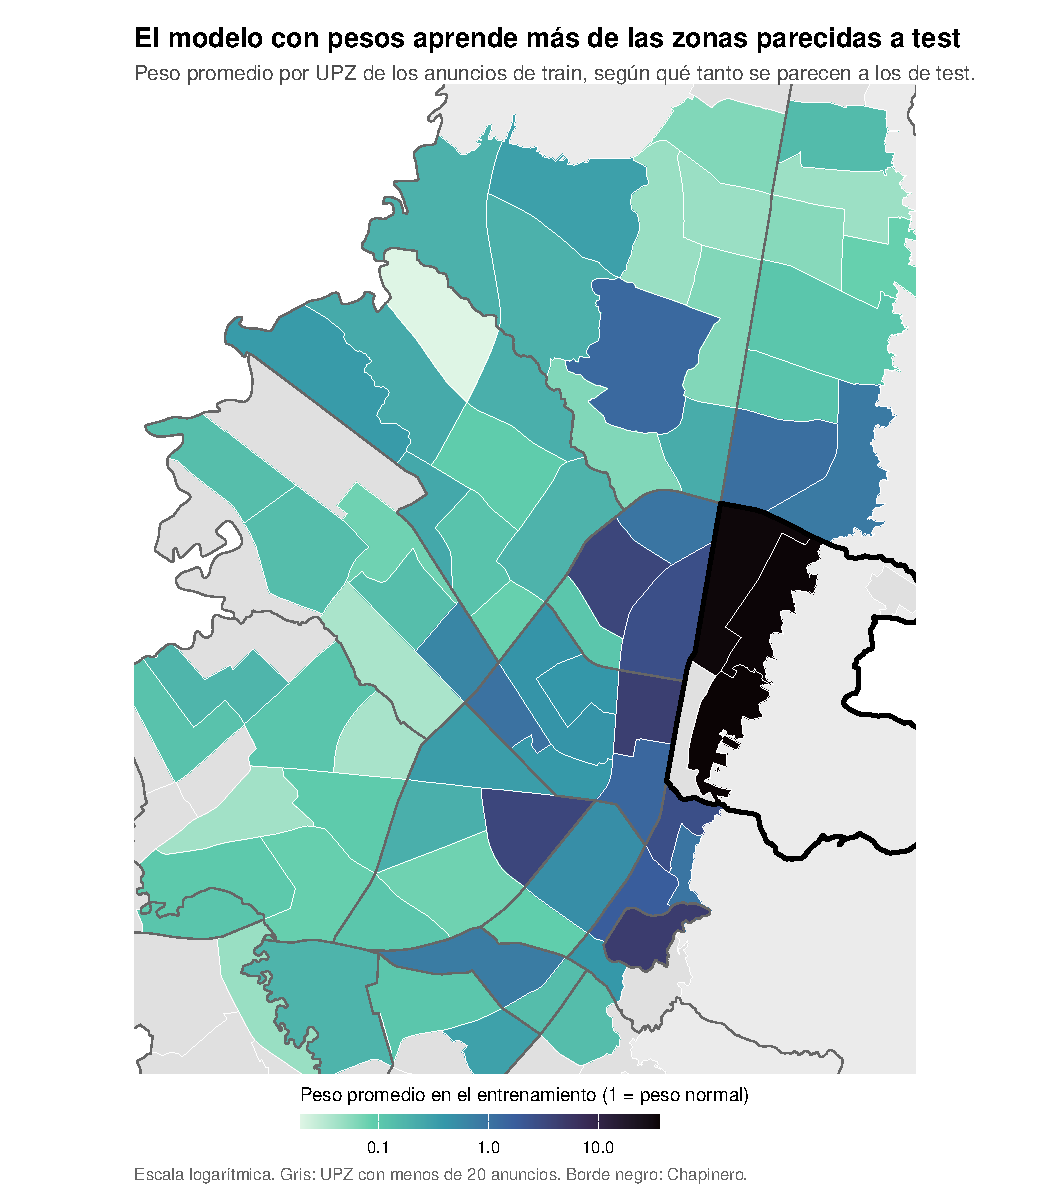
\includegraphics[height=0.82\textheight]{mapa_08_pesos_upz.pdf}
    \end{column}
    \begin{column}{0.45\textwidth}
      \begin{itemize}
        \item Un modelo aprende a distinguir los anuncios de train de los de test.
        \item Los anuncios de train que ``parecen de test'' reciben más peso al entrenar.
        \item Así el modelo dedica más esfuerzo a acertar en viviendas como las de Chapinero.
      \end{itemize}
    \end{column}
  \end{columns}
  \note{Es una forma de corregir el cambio de distribución entre train y test. El peso es la probabilidad de parecerse a test sobre la probabilidad de parecerse a train. En Kaggle los pesos ayudaron unos 3 millones en algunos pares de modelos, pero en el puntaje privado la ganancia no siempre se mantuvo: son diferencias pequeñas.}
\end{frame}
